% path for images
\graphicspath{{assets/motivation/}}

\section[Motivation]{Motivation}

%%
\begin{frame}{Why going Quantum ?}
	Until now, we’ve relied on supercomputers to solve most problems. These are very large classical computers, often with thousands of classical CPU and GPU cores. However, supercomputers aren’t very good at solving certain types of problems, which seem easy at first glance. 
\end{frame}

%%
\begin{frame}{Why going Quantum ?}
Imagine you want to seat 10 fussy people at a dinner party, where there is only one optimal seating plan out of all the different possible combinations. How many different combinations would you have to explore to find the optimal?

Can you guess how many \alert{combinations}?
\end{frame}

%% animation
\begin{frame}[<+- | only+>]{Why going Quantum ?}
	\metroset{block=fill}
	
	
	\begin{exampleblock}{For 2 people}
		2 Total combination.
	\end{exampleblock}
	

	\begin{block}{For 5 people}
		120 Total combination.
	\end{block}
	

	\begin{alertblock}{For 10 people}
		Over 3 Million of total combination!!!
	\end{alertblock}	
	
	\begin{itemize}
		\item Supercomputers don't have the working \alert{memory} to hold the myriad combinations of real world problems.
		\item Supercomputers have to analyze each combination one after another, which can take a long \alert{time}.
	\end{itemize}
\end{frame}

%% 
\begin{frame}[fragile]{Quantum Computers}
	\begin{figure}[H]
	  \centering
	    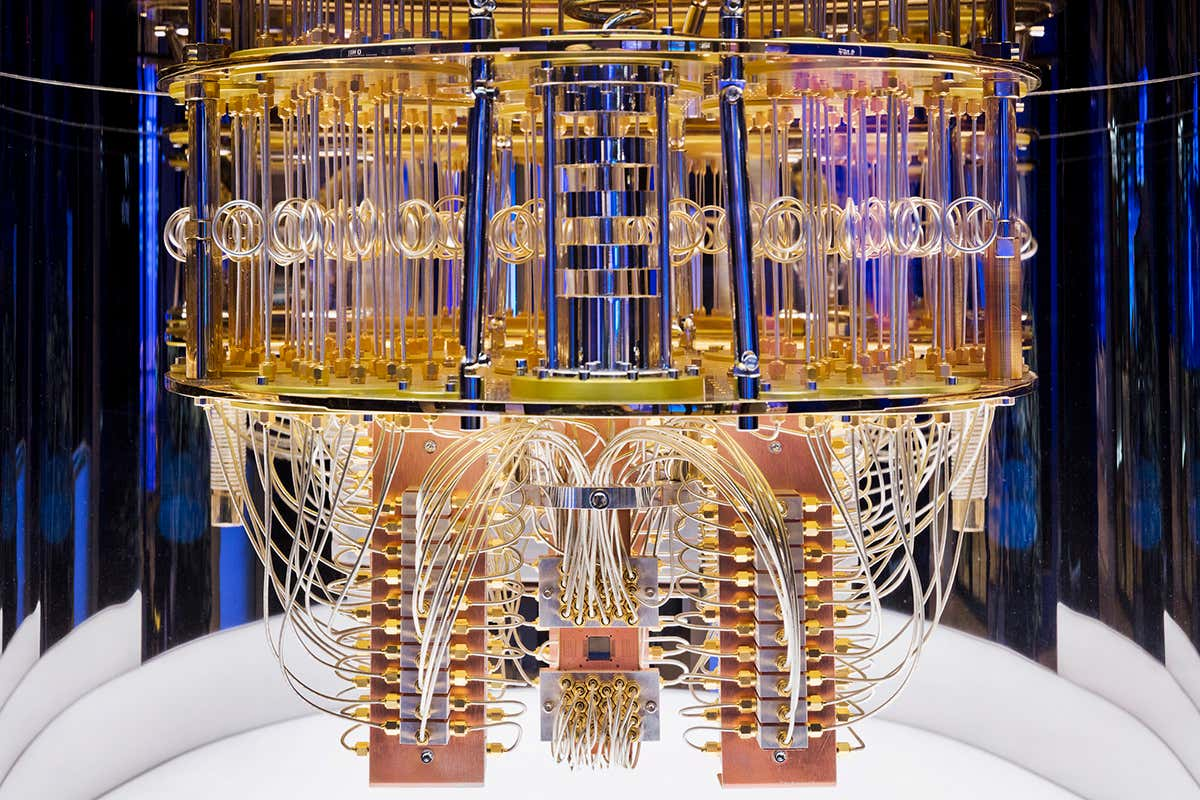
\includegraphics[width=.8\linewidth]{quantum-computer}
	    \caption{IBM's Quantum Computer}
	\end{figure}
\end{frame}

%%
\begin{frame}[fragile]{What are Quantum Computers good at ?}
	cose da dire: 
	\begin{itemize}
		\item Linear Algebra
		\item Optimization
		\item Sampling
		\item Research Algorithms
	\end{itemize}
\end{frame}

%% 
\begin{frame}[fragile]{A Growing Interest in the field}
	cose da dire: 
	\begin{itemize}
	 \item tanti framework (qiskit, pennylane, cirq, tensorflow quantum, ...)
	 \item  tanti paperi (con plot della crescita 2012-2021)
	 \item  tutti (Microsoft, Google, IBM, NVidia ... ) hanno/vogliono un computer quantistico
	 \item  tanta ricerca nel settore Quantum Programming Languages
	\end{itemize}
\end{frame}